% Options for packages loaded elsewhere
\PassOptionsToPackage{unicode}{hyperref}
\PassOptionsToPackage{hyphens}{url}
%
\documentclass[
]{article}
\usepackage{amsmath,amssymb}
\usepackage{lmodern}
\usepackage{iftex}
\ifPDFTeX
  \usepackage[T1]{fontenc}
  \usepackage[utf8]{inputenc}
  \usepackage{textcomp} % provide euro and other symbols
\else % if luatex or xetex
  \usepackage{unicode-math}
  \defaultfontfeatures{Scale=MatchLowercase}
  \defaultfontfeatures[\rmfamily]{Ligatures=TeX,Scale=1}
\fi
% Use upquote if available, for straight quotes in verbatim environments
\IfFileExists{upquote.sty}{\usepackage{upquote}}{}
\IfFileExists{microtype.sty}{% use microtype if available
  \usepackage[]{microtype}
  \UseMicrotypeSet[protrusion]{basicmath} % disable protrusion for tt fonts
}{}
\makeatletter
\@ifundefined{KOMAClassName}{% if non-KOMA class
  \IfFileExists{parskip.sty}{%
    \usepackage{parskip}
  }{% else
    \setlength{\parindent}{0pt}
    \setlength{\parskip}{6pt plus 2pt minus 1pt}}
}{% if KOMA class
  \KOMAoptions{parskip=half}}
\makeatother
\usepackage{xcolor}
\usepackage{longtable,booktabs,array}
\usepackage{calc} % for calculating minipage widths
% Correct order of tables after \paragraph or \subparagraph
\usepackage{etoolbox}
\makeatletter
\patchcmd\longtable{\par}{\if@noskipsec\mbox{}\fi\par}{}{}
\makeatother
% Allow footnotes in longtable head/foot
\IfFileExists{footnotehyper.sty}{\usepackage{footnotehyper}}{\usepackage{footnote}}
\makesavenoteenv{longtable}
\usepackage{graphicx}
\makeatletter
\def\maxwidth{\ifdim\Gin@nat@width>\linewidth\linewidth\else\Gin@nat@width\fi}
\def\maxheight{\ifdim\Gin@nat@height>\textheight\textheight\else\Gin@nat@height\fi}
\makeatother
% Scale images if necessary, so that they will not overflow the page
% margins by default, and it is still possible to overwrite the defaults
% using explicit options in \includegraphics[width, height, ...]{}
\setkeys{Gin}{width=\maxwidth,height=\maxheight,keepaspectratio}
% Set default figure placement to htbp
\makeatletter
\def\fps@figure{htbp}
\makeatother
\setlength{\emergencystretch}{3em} % prevent overfull lines
\providecommand{\tightlist}{%
  \setlength{\itemsep}{0pt}\setlength{\parskip}{0pt}}
\setcounter{secnumdepth}{-\maxdimen} % remove section numbering
\ifLuaTeX
  \usepackage{selnolig}  % disable illegal ligatures
\fi
\IfFileExists{bookmark.sty}{\usepackage{bookmark}}{\usepackage{hyperref}}
\IfFileExists{xurl.sty}{\usepackage{xurl}}{} % add URL line breaks if available
\urlstyle{same} % disable monospaced font for URLs
\hypersetup{
  pdftitle={T02 Física Universitaria - Resúmen capítulo 1 - 5},
  hidelinks,
  pdfcreator={LaTeX via pandoc}}

\title{T02 Física Universitaria - Resúmen capítulo 1 - 5}
\author{}
\date{}

\begin{document}
\maketitle

\hypertarget{mecuxe1nica}{%
\section{Mecánica}\label{mecuxe1nica}}

\hypertarget{tarea-02}{%
\subsection{Tarea 02}\label{tarea-02}}

\hypertarget{cinemuxe1tica-de-la-partuxedcula}{%
\subsection{Cinemática de la
Partícula}\label{cinemuxe1tica-de-la-partuxedcula}}

\hypertarget{fecha-de-entrega-domingo-25-de-septiembre-de-2022}{%
\subsubsection{Fecha de Entrega: Domingo 25 de septiembre de
2022}\label{fecha-de-entrega-domingo-25-de-septiembre-de-2022}}

\hypertarget{nombre-alan-yahir-juarez-rubio}{%
\subsubsection{Nombre: Alan Yahir Juarez
Rubio}\label{nombre-alan-yahir-juarez-rubio}}

\begin{center}\rule{0.5\linewidth}{0.5pt}\end{center}

\hypertarget{unidades-cantidades-fuxedsicas-y-vectores}{%
\subsection{Unidades, Cantidades Físicas y
Vectores}\label{unidades-cantidades-fuxedsicas-y-vectores}}

\hypertarget{estuxe1ndares-y-unidades}{%
\subsubsection{Estándares y unidades}\label{estuxe1ndares-y-unidades}}

\hypertarget{quuxe9-es-la-mediciuxf3n}{%
\paragraph{¿Qué es la medición?}\label{quuxe9-es-la-mediciuxf3n}}

La medición es simplemente compar unidades, comparar tamaños con otros.
Uno puede comparar el tamaño de, por ejemplo, una caja y una puerta y
puede decir que la puerta mide 5 veces el tamaño de la caja, es decir,
mide 5 cajas, pero, este sistema de medición tiene un problema, la
medida de un objeto, tal como las cajas no es la misma para todos los
ejemplares; hay cajas más pequeñas y más grandes que otras.

Para resolver este problema se desarrolló el SI (Sistema Internacional),
que establece, en base a fenómenos físicos, unidades universales tal
como el metro (para medir distancias), el segundo (para medir tiempo),
kilogramo (para medir masa), entre muchos otros. Todas estas unidades, a
comparación del ejemplo de la caja, se pueden replicar gracias a la
implementación de herramientas (regla, reloj, bascúla, etc), en la
cuales uno puede medir, puede comparar las unidades de estas con objetos
o fenómenos.

\begin{center}\rule{0.5\linewidth}{0.5pt}\end{center}

\hypertarget{prefijos-de-unidades}{%
\subsubsection{Prefijos de unidades}\label{prefijos-de-unidades}}

Tomando en cuenta las unidades fundamentales, existen notaciones que
ayudan a simplificar el entendimiento y la escritura de mediciones
grandes o pequeñas, a comparación de las unidades básicas (Fig 1).

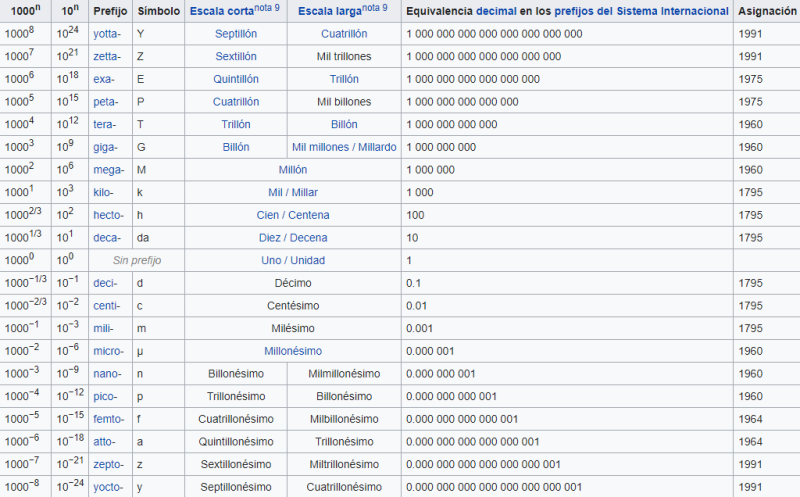
\includegraphics{L:/PCloud/Notes/Notación de Unidades de Medición.png}

Fig 1 Artículos principales: Prefijos del Sistema Internacional y
Escalas numéricas larga y corta.

\hypertarget{vectores}{%
\subsubsection{Vectores}\label{vectores}}

Un \textbf{vector} es una magnitud (tal como la rapidez, fuerza...) pero
con dirección, es decir, no solo se menciona la cantidad de unidades,
sino también la dirección a la que se emplea dicha magnitud, a la
izquierda, a la derecha hacia arriba, hacia abajo, etc. Algunas
\textbf{cantidades vectoriales} son el desplazamiento (indica el cambió
en la posición).

Si dos vectores tienen la misma dirección, son \textbf{paralelos}; si
tienen la misma magnitud y dirección, son iguales y se representa como
{\(\overset{\rightarrow}{A} = \overset{\rightarrow}{B}\)}; en cambio, si
tienen la misma magnitud, pero no la misma dirección, no son iguales. En
caso de ser iguales en magnitud, pero en direccción opuesta se
representaría como
{\(\overset{\rightarrow}{A} = - \overset{\rightarrow}{B}\)}. Dos
vectores con distinta o igual magnitud, pero en dirección opuestas se
les dice que son \textbf{antiparalelos}.

\hypertarget{suma-de-vectores}{%
\paragraph{Suma de vectores}\label{suma-de-vectores}}

\begin{longtable}[]{@{}lll@{}}
\toprule()
Suma de vectores & Caso & Conversión a magnitud \\
\midrule()
\endhead
{\(\overset{\rightarrow}{C} = \overset{\rightarrow}{A} + \overset{\rightarrow}{B}\)}
& cuando {\(\overset{\rightarrow}{A}\)} y {\(\overset{\rightarrow}{B}\)}
son \textbf{paralelos} entre sí &
{\(\overset{\rightarrow}{C} = A + B\)} \\
{\(\overset{\rightarrow}{C} = \overset{\rightarrow}{A} + \overset{\rightarrow}{B}\)}
& cuando {\(\overset{\rightarrow}{A}\)} y {\(\overset{\rightarrow}{B}\)}
son \textbf{antiparalelos} entre sí &
{\(\overset{\rightarrow}{C} = \text{|}A - B\text{|}\)} \\
\bottomrule()
\end{longtable}

\hypertarget{suma-de-muxe1s-de-dos-vectores}{%
\paragraph{Suma de más de dos
vectores}\label{suma-de-muxe1s-de-dos-vectores}}

Primero se suma dos vectores cualquiera y la resultante sumarla con el
tercero (Caso 1) o, en dado caso la resultante de la suma del siguiente
par de vectores (Caso 2)

Caso
1{\[\overset{\rightarrow}{R} = (\overset{\rightarrow}{A} + \overset{\rightarrow}{B}) + \overset{\rightarrow}{C} = \overset{\rightarrow}{D} + \overset{\rightarrow}{C}\]}

Caso
2{\[\overset{\rightarrow}{R} = (\overset{\rightarrow}{A} + \overset{\rightarrow}{B}) + (\overset{\rightarrow}{C} + \overset{\rightarrow}{D}) = \overset{\rightarrow}{E} + \overset{\rightarrow}{F}\]}

Cabe mencionar que no es necesario dibujar los vectores resultantes
({\(\overset{\rightarrow}{E}\)} y {\(\overset{\rightarrow}{F}\)}) Caso
2, sino solo al vector resultante {\(\overset{\rightarrow}{R}\)}

\hypertarget{componente-de-vectores}{%
\paragraph{Componente de vectores}\label{componente-de-vectores}}

Por definición, cada vector componente tiene la dirección de un eje de
coordenadas, por lo que solo necesitas un número para describirlo. Si el
vector compenente {\({\overset{\rightarrow}{A}}_{x}\)} apunta hacia la
dirección {\(x\)} positiva, definimos el número {\(A_{x}\)}; si
{\({\overset{\rightarrow}{A}}_{x}\)} apunta a la dirección {\(x\)}
negativa, {\(A_{x}\)} es igual al negativo de dicha magnitud, teniento
presente que la magnitud en sí de un vector nunca es negativa. Definimos
el número de {\(A_{y}\)} del mismo modo. {\(A_{x}\)} y {\(A_{y}\)} son
las \textbf{componentes} de {\(\overset{\rightarrow}{A}\)}

\begin{center}\rule{0.5\linewidth}{0.5pt}\end{center}

{\(\frac{A_{x}}{A} = \cos\theta\)} y
{\(\frac{A_{y}}{A} = \sin\theta\)}\\
{\(A_{x} = A\cos\theta\)} y {\(A_{y} = A\sin\theta\)}

Estas ecuaciones son correctas si solo el ángulo {\(\theta\)} se mide
desde el eje {\(x\)} positivo

También se puede usar el teorema de pitagoras para obtener la magnitud y
la dirección a partir de las componentes.

{Ⅱ\[A = \sqrt{{A_{x}}^{2} + {A_{y}}^{Ⅱ}}\]}

\begin{center}\rule{0.5\linewidth}{0.5pt}\end{center}

\hypertarget{vectores-unitarios}{%
\subsubsection{Vectores unitarios}\label{vectores-unitarios}}

Un \textbf{vector unitario} es un vector cont magnitud 1, sin unidades.
Sú único fin es describir una dirección en el espacio. En estos vectores
se incluye un acento circunplejo (\^{}) encima de estos.

\begin{longtable}[]{@{}ccc@{}}
\toprule()
Vector unitario & Eje & Su relación con los componentes de un vector \\
\midrule()
\endhead
{\(\hat{\imath}\)} & {\(+ x\)} &
{\({\overset{\rightarrow}{A}}_{x} = A_{x}\hat{\imath}\)} \\
{\(- \hat{\imath}\)} & -x &
{\({\overset{\rightarrow}{A}}_{x} = A_{x} - \hat{\imath}\)} \\
{\(\hat{\jmath}\)} & {\(+ y\)} &
{\({\overset{\rightarrow}{A}}_{y} = A_{y}\hat{\jmath}\)} \\
{\(- \hat{\jmath}\)} & {\(- y\)} &
{\({\overset{\rightarrow}{A}}_{y} = A_{y} - \hat{\jmath}\)} \\
{\(\hat{k}\)} & {\(+ z\)} &
{\({\overset{\rightarrow}{A}}_{z} = A_{z}\hat{k}\)} \\
-{\(\hat{k}\)} & {\(- z\)} &
{\({\overset{\rightarrow}{A}}_{z} = A_{z} - \hat{k}\)} \\
\bottomrule()
\end{longtable}

Cuando representamos dos vectores {\(\overset{\rightarrow}{A}\)} y
{\(\overset{\rightarrow}{B}\)} en términos de sus componentes, podemos
representar la resultante como {\(\overset{\rightarrow}{R}\)} usando
vectores unitarios de la siguiente manera:

{\(\overset{\rightarrow}{A} = A_{x}\hat{\imath} + A_{y}\hat{\jmath} + A_{z}\hat{k}\)}\\
{\(\overset{\rightarrow}{B} = B_{x}\hat{\imath} + B_{y}\hat{\jmath} + B_{z}\hat{k}\)}

{\(\overset{\rightarrow}{R} = \overset{\rightarrow}{A} + \overset{\rightarrow}{B}\)}\\
{\(= (A_{x} + B_{x} + C_{x})\hat{\imath} + (A_{y} + B_{y} + C_{y})\hat{\jmath} + (A_{z} + B_{z} + C_{z})\hat{k}\)}\\
{\(\overset{\rightarrow}{R} = R_{x}\hat{\imath} + R_{y}\hat{\jmath} + + R_{z}\hat{k}\)}

\begin{center}\rule{0.5\linewidth}{0.5pt}\end{center}

\hypertarget{productos-de-vectores}{%
\subsubsection{Productos de vectores}\label{productos-de-vectores}}

{\[\overset{\rightarrow}{A} \cdot \overset{\rightarrow}{B} = AB\cos\phi = |\overset{\rightarrow}{A}||\overset{\rightarrow}{B}|\cot\phi\]}

donde {\(\phi\)} está entre 0° y 180°

Si {\(\phi\)} está entre 0° y 90°, el producto escalar será postivo, y
negativo si {\(\phi\)} está entre 90° y 180°. El producto escalar de dos
vectores pependiculas siempre es cero.

{\(\hat{\imath} \cdot \hat{\imath} = \hat{\jmath} \cdot \hat{\jmath} = \hat{k} \cdot \hat{k} = (1)(1)\cos 0 = 1\)}\\
{\(\hat{\imath} \cdot \hat{\jmath} = \hat{\imath} \cdot \hat{k} = \hat{\jmath} \cdot \hat{k} = (1)(1)\cos 90 = 0\)}

{\(\overset{\rightarrow}{A} \cdot \overset{\rightarrow}{B} = (A_{x}\hat{\imath} + A_{y}\hat{\jmath} + A_{z}\hat{k}) \cdot (B_{x}\hat{\imath} + B_{y}\hat{\jmath} + B_{z}\hat{k})\)}

{\(= A_{x}\hat{\imath} \cdot B_{x}\hat{\imath} + A_{x}\hat{\imath} \cdot B_{y}\hat{\jmath} + A_{x}\hat{\imath} \cdot B_{z}\hat{k}\)}\\
{\(+ A_{y}\hat{\jmath} \cdot B_{x}\hat{\imath} + A_{y}\hat{\jmath} \cdot B_{y}\hat{\jmath} + A_{y}\hat{\jmath} \cdot B_{z}\hat{k}\)}\\
{\(+ A_{z}\hat{k} \cdot B_{x}\hat{\imath} + A_{z}\hat{k} \cdot B_{y}\hat{\jmath} + A_{z}\hat{k} \cdot B_{z}\hat{k}\)}

{\(= A_{x}B_{x}\hat{\imath} \cdot \hat{\imath} + A_{x}B_{y}\hat{\imath} \cdot \hat{\jmath} + A_{x}B_{z}\hat{\imath} \cdot \hat{k}\)}\\
{\(+ A_{y}B_{x}\hat{\jmath} \cdot \hat{\imath} + A_{y}B_{y}\hat{\jmath} \cdot \hat{\jmath} + A_{y}B_{z}\hat{\jmath} \cdot \hat{k}\)}\\
{\(+ A_{z}B_{x}\hat{k} \cdot \hat{\imath} + A_{z}B_{y}\hat{k} \cdot \hat{\jmath} + A_{z}B_{z}\hat{k} \cdot \hat{k}\)}

{\(\overset{\rightarrow}{A} \cdot \overset{\rightarrow}{B} = A_{x}B_{x} + A_{y}B_{y} + A_{z}B_{z}\)}

\begin{center}\rule{0.5\linewidth}{0.5pt}\end{center}

\textbackslash pagebreak

\hypertarget{movimiento-en-luxednea-recta}{%
\subsection{Movimiento en Línea
Recta}\label{movimiento-en-luxednea-recta}}

\hypertarget{desplazamiento-tiempo-y-velocidad-media}{%
\subsubsection{Desplazamiento, tiempo y velocidad
media}\label{desplazamiento-tiempo-y-velocidad-media}}

Para medir el movimiento de una \textbf{partícula} es en términos del
cambio de posición a lo largo de un intérvalo de tiempo.

La componente {\(x\)} del desplazamientos es simplemente el cambio de
valor de {\(x\)}.

{\(\Delta x = x_{2} - x_{1}\)}

{\[v_{\text{med} - x} = \frac{x_{2} - x_{1}}{t_{2} - t_{1}} = \frac{\Delta x}{\Delta t}\]}Una
velocidad media positiva o negativa no representa un movimiento hacia la
derecha o hacia la izquierda. Esto solo depende de hacia qué lado
establecimos el eje {\(+ x\)}.

\begin{center}\rule{0.5\linewidth}{0.5pt}\end{center}

\hypertarget{velocidad-instuxe1ntanea}{%
\subsubsection{Velocidad instántanea}\label{velocidad-instuxe1ntanea}}

Para describir el movimiento de una \textbf{partícula} con mayor detalle
es necesario definir la velocidad en cualquier instante específico esto
se le llama \textbf{velocidad instántanea}. Para calcularla, primero
debemos calcular la velocidad media

{\(v_{x} = \lim\limits_{\Delta r \rightarrow 0}\frac{\Delta x}{\Delta t} = \frac{dx}{dt}\)}

Como {\(\Delta t\)} es siempre positivo, {\(v_{x}\)} tiene el mismo
signo que {\(\Delta x\)}.

Como en este caso la partícula solo tiene movimiento en el eje {\(x\)}
o, dicho de otra manera, {\(x\)} es el único componente de la velocidad
media, los componentes {\(y\)} y {\(z\)} son igual a cero. Entonces en
estos tipos de casos se puede decir que {\(v_{x}\)} es igual a la
velocidad instántanea.

\begin{center}\rule{0.5\linewidth}{0.5pt}\end{center}

\hypertarget{aceleraciuxf3n-media-e-instantuxe1nea}{%
\subsubsection{Aceleración media e
instantánea}\label{aceleraciuxf3n-media-e-instantuxe1nea}}

\hypertarget{aceleraciuxf3n-media}{%
\paragraph{Aceleración media}\label{aceleraciuxf3n-media}}

{\(a_{\text{med} - x} = \frac{v_{2_{x}} - v_{1_{x}}}{t_{2} - t_{1}} = \frac{\Delta v_{x}}{\Delta t}\)}

\hypertarget{aceleraciuxf3n-instuxe1ntanea}{%
\paragraph{Aceleración
instántanea}\label{aceleraciuxf3n-instuxe1ntanea}}

{\(a_{x} = \lim{\Delta r \rightarrow 0}\frac{\Delta v_{x}}{\Delta t} = \frac{dv_{x}}{dt}\)}

\begin{center}\rule{0.5\linewidth}{0.5pt}\end{center}

\hypertarget{cuerpos-en-cauxedda-libre}{%
\subsubsection{Cuerpos en caída libre}\label{cuerpos-en-cauxedda-libre}}

La aceleración constante de un cuerpo en caída libre se llama
\textbf{aceleración debida a la gravedad} y denotamos su magnitud con
{\(g\)}, el cual tiene un valor aproximado de
{\(9.80665\text{~m/s}^{2}\)}, el cual se suele manejar como
{\(9.8\text{~m/s}^{2}\)} o, para simples explicaciones como
{\(10\text{~m/s}^{2}\)}. El valor exacto varía según el lugar, pero en
la mayoria de los casos no es necesario calcularlo debido a que la tasa
de error es relativamente insignificativa.

\begin{center}\rule{0.5\linewidth}{0.5pt}\end{center}

\textbackslash pagebreak

\hypertarget{movimiento-en-dos-o-tres-dimensiones}{%
\subsection{Movimiento en Dos o Tres
Dimensiones}\label{movimiento-en-dos-o-tres-dimensiones}}

\hypertarget{vectores-de-posiciuxf3n-y-velocidad}{%
\subsubsection{Vectores de posición y
velocidad}\label{vectores-de-posiciuxf3n-y-velocidad}}

{\(\overset{\rightarrow}{r} = x\hat{\imath} + y\hat{\jmath} + z\hat{k}\)}\\
{\({\overset{\rightarrow}{v}}_{\text{m}ed} = \frac{{\overset{\rightarrow}{r}}_{2} - {\overset{\rightarrow}{r}}_{1}}{t^{2} - t_{1}} = \frac{\Delta\overset{\rightarrow}{r}}{\Delta t}\)}\\
{\(\overset{\rightarrow}{v} = \lim\limits_{\Delta r \rightarrow 0}\frac{\Delta\overset{\rightarrow}{r}}{\Delta t} = \frac{d\overset{\rightarrow}{r}}{dt}\)}\\
{\(\overset{\rightarrow}{v} = \frac{d\overset{\rightarrow}{r}}{dt} = \frac{dx}{dt}\hat{\imath} + \frac{dy}{dt}\hat{\jmath} + \frac{dz}{dt}\hat{k}\)}\\
{\(|\overset{\rightarrow}{v}| = v = \sqrt{{v_{x}}^{2} + {v_{y}}^{2} + {v_{z}}^{2}}\)}\\
{\(\tan\alpha = \frac{v_{y}}{v_{x}}\)}

\begin{center}\rule{0.5\linewidth}{0.5pt}\end{center}

\hypertarget{el-vector-de-aceleraciuxf3n}{%
\subsubsection{El vector de
aceleración}\label{el-vector-de-aceleraciuxf3n}}

{\({\overset{\rightarrow}{a}}_{\text{m}ed} = \frac{{\overset{\rightarrow}{v}}_{2} - {\overset{\rightarrow}{v}}_{1}}{t^{2} - t_{1}} = \frac{\Delta\overset{\rightarrow}{v}}{\Delta t}\)}\\
{\(\overset{\rightarrow}{v} = \lim\limits_{\Delta v \rightarrow 0}\frac{\Delta\overset{\rightarrow}{v}}{\Delta t} = \frac{d\overset{\rightarrow}{r}}{dt}\)}\\
{\(\overset{\rightarrow}{a} = \frac{dv_{x}}{dt}\hat{\imath} + \frac{dv_{y}}{dt}\hat{\jmath} + \frac{dv_{z}}{dt}\hat{k}\)}\\
{\(\overset{\rightarrow}{a} = \frac{d^{2}x}{dt}\hat{\imath} + \frac{d^{2}y}{dt}\hat{\jmath} + \frac{d^{2}z}{dt}\hat{k}\)}

\begin{center}\rule{0.5\linewidth}{0.5pt}\end{center}

\hypertarget{movimiento-de-proyectiles}{%
\subsubsection{Movimiento de
proyectiles}\label{movimiento-de-proyectiles}}

Un \textbf{proyectil} es un cuerpo que recibe una velocidad inicial y
luego sigue una trayectoria determinada totalmente por los efectos de la
aceleración gravitacional y la resistencia del aire. En el movimiento de
proyectiles no se toma en cuenta la resistencia del aire

Para analizar el movimiento de un proyectil, este se divide en 2 casos;
para el componente {\(x\)} movimiento rectilineo uniforme, debido a que
la aceleración de este componente es 0 y para el eje {\(y\)} caída
libre, debido a que la aceleración del componente de {\(y\)} es igual a
{\(- g\)}, es decir, {\(- 9.81\text{~m/s}^{2}\)}, negativa porque el
objeto va descendiendo, se dirige hacia el eje {\(- y\)}.

{\(v_{x} = v_{0_{x}}\)}\\
{\(x = x_{0} + v_{0_{x}}t\)}

{\(v_{y} = vv_{0_{y}} - gt\)}\\
{\(y = y_{0} + v_{0_{y}}t - \frac{1}{2}gt^{2}\)}

{\(x = (v_{0}\cos\alpha_{0})\)}\\
{\(y = (v_{0}\sin\alpha_{0})t - \frac{1}{2}gt^{2}\)}\\
{\(v_{x} = v_{0}\cos\alpha_{0}\)}\\
{\(v_{y} = v_{0}\sin\alpha_{0} - gt\)}

{\(r = \sqrt{x^{2} + y^{2}}\)}\\
{\(v = \sqrt{{v_{x}}^{2} + {v_{y}}^{2}}\)}\\
{\(\tan\alpha = \frac{v_{y}}{v_{x}}\)}\\
{Ⅱ\(y = (\tan\alpha_{0})x - \frac{5}{2{v_{0}}^{2}\cos^{2}\alpha_{0}}x^{Ⅱ}\)}\\
{\(y = bx - cx^{2}\)} tarts

\begin{center}\rule{0.5\linewidth}{0.5pt}\end{center}

\hypertarget{movimiento-circular-uniforme}{%
\subsubsection{Movimiento circular
uniforme}\label{movimiento-circular-uniforme}}

{\(\frac{\mid \Delta\overset{\rightarrow}{v} \mid}{v_{1}} = \frac{\Delta s}{R}\)}
o
{\(\mid \Delta\overset{\rightarrow}{v}\operatorname{\mid=}\frac{v_{1}}{R}\Delta s\)}

{\(a_{\text{med}} = \frac{\mid \Delta\overset{\rightarrow}{v} \mid}{\Delta t} = \frac{v_{1}}{R}\frac{\Delta s}{\Delta t}\)}

{\(a_{\text{med}} = \lim\limits_{\delta t \rightarrow 0}\frac{v_{1}}{R}\frac{\Delta s}{\Delta t} = \frac{v_{1}}{R}\lim\limits_{\Delta t \rightarrow 0}\frac{\Delta s}{\Delta t}\)}

{\(v = \frac{2\pi R}{T}\)}

{\(a_{\text{rad}} = \frac{4\pi^{2}R}{T^{2}}\)}

\begin{center}\rule{0.5\linewidth}{0.5pt}\end{center}

\hypertarget{movimiento-circular-no-uniforme}{%
\subsubsection{Movimiento circular no
uniforme}\label{movimiento-circular-no-uniforme}}

{\(a_{\text{rad}} = \frac{v^{2}}{R}\)} y
{\(a_{\tan} = \frac{d \mid \overset{\rightarrow}{v} \mid}{dt}\)}

\begin{center}\rule{0.5\linewidth}{0.5pt}\end{center}

\hypertarget{velocidad-relativa-en-una-dimensiuxf3n}{%
\subsubsection{Velocidad relativa en una
dimensión}\label{velocidad-relativa-en-una-dimensiuxf3n}}

{\(x_{P/A} = x_{P/B} + x_{B/A}\)}

{\(\frac{dx_{P/A}}{dt} = \frac{dx_{P/B}}{dt} + \frac{dx_{B/A}}{dt}\)}

{\(v_{P/A - x} = v_{P/B - x} + vx_{B/A - x}\)}

\begin{center}\rule{0.5\linewidth}{0.5pt}\end{center}

\hypertarget{velocidad-relativa-en-dos-o-tres-dimensiones}{%
\subsubsection{Velocidad relativa en dos o tres
dimensiones}\label{velocidad-relativa-en-dos-o-tres-dimensiones}}

{\({\overset{\rightarrow}{r}}_{P/A} = {\overset{\rightarrow}{r}}_{P/B} + {\overset{\rightarrow}{r}}_{B/A}\)}\\
{\({\overset{\rightarrow}{v}}_{P/A} = {\overset{\rightarrow}{v}}_{P/B} + {\overset{\rightarrow}{v}}_{B/A}\)}

{\(\frac{dx_{P/A}}{dt} = \frac{dx_{P/B}}{dt} + \frac{dx_{B/A}}{dt}\)}

{\(v_{P/A - x} = v_{P/B - x} + vx_{B/A - x}\)}\\
{\(\tan\phi = \frac{v_{P/B}}{v_{B/A}}\)}

\begin{center}\rule{0.5\linewidth}{0.5pt}\end{center}

\textbackslash pagebreak

\hypertarget{leyes-del-movimiento-de-newton}{%
\subsection{Leyes del Movimiento de
Newton}\label{leyes-del-movimiento-de-newton}}

\hypertarget{superposiciuxf3n-de-fuerzas}{%
\subsubsection{Superposición de
fuerzas}\label{superposiciuxf3n-de-fuerzas}}

{\(\overset{\rightarrow}{R} = {\overset{\rightarrow}{F}}_{1} + {\overset{\rightarrow}{F}}_{2} + {\overset{\rightarrow}{F}}_{1} + \cdots = \sum\overset{\rightarrow}{F}\)}

{\(R_{x} = \sum F_{x}\)} y {\(R_{y} = \sum F_{y}\)}

{\(R = \sqrt{{R_{x}}^{2} + {R_{y}}^{2} + {R_{z}}^{2}}\)}

\begin{center}\rule{0.5\linewidth}{0.5pt}\end{center}

\hypertarget{primera-ley-de-newton}{%
\subsubsection{Primera ley de Newton}\label{primera-ley-de-newton}}

{\(\sum\overset{\rightarrow}{F} = {\overset{\rightarrow}{F}}_{1} + {\overset{\rightarrow}{F}}_{2} = {\overset{\rightarrow}{F}}_{1} + ( - {\overset{\rightarrow}{F}}_{2}) = 0\)}\\
{\(\sum\overset{\rightarrow}{F} = 0\)}\\
{\(\sum{\overset{\rightarrow}{F}}_{x} = 0\)}
{\(\sum{\overset{\rightarrow}{F}}_{y} = 0\)}

\begin{center}\rule{0.5\linewidth}{0.5pt}\end{center}

\hypertarget{segunda-ley-de-newton}{%
\subsubsection{Segunda ley de Newton}\label{segunda-ley-de-newton}}

{\(m = \frac{\mid \sum\overset{\rightarrow}{F} \mid}{a}\)} o
{\(\mid \sum\overset{\rightarrow}{F}\operatorname{\mid=}ma\)} o
{\(a = \frac{\mid \sum\overset{\rightarrow}{F} \mid}{m}\)}\\
{\(m_{1}a_{1} = m_{2}a_{2}\)}

{\(\frac{m_{2}}{m_{1}} = \frac{a_{1}}{a_{2}}\)}

{\(\sum\overset{\rightarrow}{F} = m\overset{\rightarrow}{a}\)}

{\(\overset{\rightarrow}{a} = \frac{\sum\overset{\rightarrow}{F}}{m}\)}

\begin{center}\rule{0.5\linewidth}{0.5pt}\end{center}

\hypertarget{masa-y-peso}{%
\subsubsection{Masa y peso}\label{masa-y-peso}}

{\(w = mg\)}\\
{\(\overset{\rightarrow}{w} = m\overset{\rightarrow}{g}\)}

\begin{center}\rule{0.5\linewidth}{0.5pt}\end{center}

\hypertarget{tercera-ley-de-newton}{%
\subsubsection{Tercera ley de Newton}\label{tercera-ley-de-newton}}

{\({\overset{\rightarrow}{F}}_{A\text{~sobre~}B} = {\overset{\rightarrow}{F}}_{B\text{~sobre~}A}\)}

\begin{center}\rule{0.5\linewidth}{0.5pt}\end{center}

\textbackslash pagebreak

\hypertarget{aplicaciuxf3n-de-las-leyes-de-newton}{%
\subsection{Aplicación de las Leyes de
Newton}\label{aplicaciuxf3n-de-las-leyes-de-newton}}

\hypertarget{fuerzas-de-fricciuxf3n}{%
\subsubsection{Fuerzas de fricción}\label{fuerzas-de-fricciuxf3n}}

\hypertarget{fricciuxf3n-cinuxe9tica-y-estuxe1tica}{%
\paragraph{Fricción cinética y
estática}\label{fricciuxf3n-cinuxe9tica-y-estuxe1tica}}

{µ\(f_{k} = µ_{k}n\)}\\
{µ\(f_{s} \leq µ_{s}n\)}

\begin{center}\rule{0.5\linewidth}{0.5pt}\end{center}

\textbackslash pagebreak

\hypertarget{glosario}{%
\subsection{Glosario}\label{glosario}}

\textbf{Teoría}: Explicación de fenómenos naturales basada en
observaciones y en los principios fundamentales observados

\textbf{Partícula:} punto de referencia que representa a un objeto en un
sistema de coordenadas.

\textbf{Aceleración}: cambio de velocidad respecto al tiempo.

\begin{center}\rule{0.5\linewidth}{0.5pt}\end{center}

\textbackslash pagebreak

\hypertarget{bibliografuxeda}{%
\subsection{Bibliografía}\label{bibliografuxeda}}

\begin{itemize}
\tightlist
\item
  Sears, F. W., Zemansky M. W., Young, H. D., Freedman, R. A., Ford A.
  L. (2004). Wesley, P. A (Ed.). \emph{Física Universitaria}
  (11{\(^{\text{a}}\)} ed, Vol. 1). México. Pearson Educación.
  \url{https://ebookcentral-proquest-com.wdg.biblio.udg.mx:8443/lib/wdgbiblio/reader.action?docID=5134269\&ppg}
\end{itemize}

\end{document}
